The HMM model described in the Chapter \ref{c02} is uses the divide and conquer strategy which has been defined as a generative method in which we use the smaller components represented by the HMM to learn the entire speech process.   As also previously mentioned this is referred to as the bottom-up strategy.  The discriminative method however uses the opposite mechanism.  Rather than using the building blocks of speech to determine speech parameters of a HMM, the discriminative strategy determines the posterior probability directly using the joint probability distribution of the parameters involved in the discriminative process.  The discriminative parameters are discussed in this section where the Neural network discriminative approach is described beginning with the architecture.

\section{Neural network architecture}

The building block of a neural network simulates a combination of two consecutive linear and non-linear operations having many inputs interconnected with the linear portion of the network.  This rudimentary structure is described by McCullough and Pitts (1942) in  \cite{cowan1990discussion} as the Perceptron in figure \ref{fig_3_1_ptron} 

\begin{figure}
\centering
  % Requires \usepackage{graphicx}
  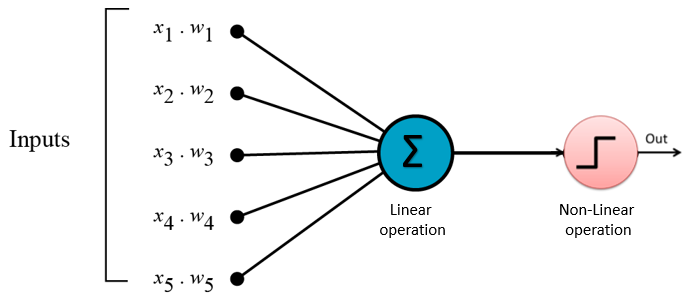
\includegraphics[width=7cm]{thesis/images/ptron2.png}\\
  \caption{Perceptron} \label{fig_3_1_ptron}
\end{figure}

The linear operation is the sum of the products of the input feature and a  weight vector set.  This vector sum of products is referred to as an affine transformation or operation.  The non linear operation is the given by any one of a selection of nonlinear functions.  In  figure \ref{fig_3_2_nn} this is shown as a step function.  The step function is activated (becomes 1) whenever the output of the linear function is above a certain threshold, otherwise remains at 0.  A simple neural network of perceptrons is formed by stacking the perceptrons into an interconnected layer as shown in the figure \ref{fig_3_2_nn}  :

\begin{figure}
\centering
  % Requires \usepackage{graphicx}
  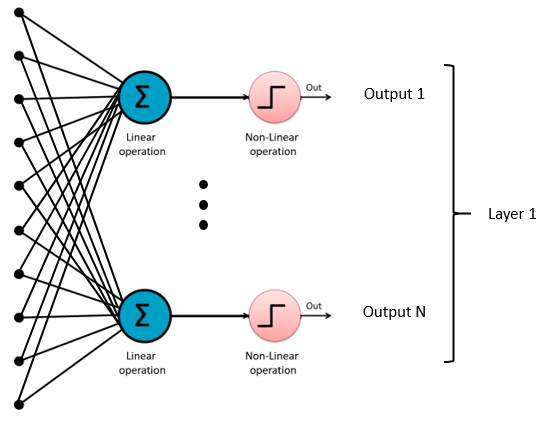
\includegraphics[width=7cm]{thesis/images/ptron3.png}\\
  \caption{Neural network} \label{fig_3_2_nn}
\end{figure}

In this regime each combination of linear operation followed by a non linear operation is called a neuron and the total number of neurons in the layer formed is termed as $M$-number of neurons in the layer.

\subsection{Multi-layer Perceptron (MLP)}
The multilayer Perceptron or MLP extends the basic Perceptron structure by adding one or more hidden layers.  These hidden layers comprise the outputs of one layer becoming the input of the next layer. In the simplest case having one hidden layer, the output of layer 1 becomes the input of the final output layer.  In comparison, the Perceptron is a one dimensional structure having one or more linear and non linear combination outputs, while the multilayer Perceptron is a 2-dimensional structure having one or more hidden layers of $N$ linear and non-linear combination outputs.  Mathematically speaking the output of each layer of an MLP having $N$ inputs and $M$ neurons is given by
\begin{equation}
z_j=h(b_j)=\frac{1}{ 1+e^{-b_j}} 
\label{eqn_c3_nn_01}
\end{equation}
 is the non-linear function while  is the linear function given by:
\begin{equation}
b_j=\sum_{i=0}^Nw_{ji}^{(1)}\qquad j=1,2,\dots,M
\label{eqn_c3_nn_02}
\end{equation}

For each layer in the MLP, the zeroth input value $x_0$ is 1 indicating a bias term.  This bias term is used in the neural network to ensure regularised and expected behaviour of the neural network.  In this example the non-linear step function is given by a more complex exponential.  In the next section the nonlinear functions for a multilayer Perceptron is derived.

\subsection{Sigmoid and soft-max Activation Function}
The combination of the linear function and the non linear function in the neural network could be said to be transformation of an algebraic problem to a probabilistic function.  In this case the "step" function is a squashing sigmoid-shaped function that converts the inputs into a Naive Bayes function evaluating the probability that an output belongs to any of the output classes $(C_y)$ given the data $(\mathbf{x})$.
\begin{equation}
p(C_1|\mathbf{x})=f(a)=f(\mathbf{w^\top x}+w_0)
\label{eqn_c3_nn_02}\end{equation}
In a two class problem with classes $C_1$ and $C_2$, the posterior probability of class $C_1$ is expressed using Bayes’s theorem
\begin{equation}
p(C_1|\mathbf{x})=\frac{p(\mathbf{x}|C_1)p(C_1)}{p(x|C_1)p(C_1)+p(\mathbf{x}|C_2)p(C_2)}
\label{eqn_c3_nn_03}\end{equation}
Dividing through by $p(\mathbf{x}|C_1)p(C_1)$ gives us
\begin{equation}
p(C_1|\mathbf(x)=\frac{1}{1+\frac{p(\mathbf{x}|C_1)p(C_1)}{p(\mathbf{x}|C_2)p(C_2)}}
\label{eqn_c3_nn_04}\end{equation}

If we define the ratio of the log posterior probabilities as
\begin{equation}
a=\ln\frac{p(\mathbf{x}|C_1)p(C_1)}{p(\mathbf{x}|C_2)p(C_2)}
\label{eqn_c3_nn_05}\end{equation}
If we substitute back into (4) we have:

\begin{equation}p(C_1|\mathbf{x})=f(a)=\frac{1}{1+e^{-a}}
\label{eqn_c3_nn_06}
\end{equation}

Here $a=\mathbf{w^\top x}=w_0$.  Thus the activation for the non-linear function is driven by the probability of the data to give the output class.  The probabilistic function here is called a sigmoid function due to the s-shaped graph that is plotted by the function.

Rather than using the sigmoid function for multi-class classification a similar soft max function is derived by using the log probability of classes. If $a_k=\ln(p(\mathbf{x}|C_k)p(C_k))$ then:
\begin{equation}
y_k=p(C_k|\mathbf{x})=\frac{e^{a_k}}{\Sigma_{\ell=1}^K e^{a_\ell}}
\label{eqn_c3_nn_07}\end{equation}
\begin{equation}
a_k=\sum_{i=0}^dw_{ki}x_i
\label{eqn_c3_nn_08}\end{equation}

Recall that in the generative classification method the problem is divided into sub problems by using the conditional probability, while in the discriminative approach the joint probability is determined by looking at the data directly.  This is what $p(C_k|\mathbf{x})$ represents.  However also, recall that we still need to determine the correct probability distribution represented by the data.  This is achieved by determining the values of the weights of the linear operation.  In the next section a method known as back propagation is discussed.  Back propagation is the training algorithm used to determine the weight vector of all the layers in the neural network.  Back propagation is an extension of the Gradient descent algorithm.

\subsection{Back propagation algorithm (backprop)}
In the previous section, the neural network architecture has been described as having $N$ inputs $M$ neurons and $L$ layers. Each layer comprises $M$ neurons of a maximum of $N$ inputs times $M$ neurons interconnections which embodies the inner product of the inputs and unknown set of weights. The output of this inner product is then passed to a logistic squashing function that results output probabilities.  The discriminative process is used here to determine the correct combination of weight vectors that accurately describe the training data.  For neural networks, the weight vectors at each layer are determined through propagating the errors back through each preceding layer and adjusting the weights according to the errors propagated each time a batch of the data is processed.  This process of continuously adjusting weights from back propagation continues until all the data is processed and a steady state has been reached.  The steady state refers to the fact that the error has reached a steady and/or acceptable negligible value.  This is often referred to in machine learning as convergence \citep{boden2002guide}.

\subsubsection{Gradient Descent}
The last section ended stating that the back-propagation algorithm is an extension of the gradient descent algorithm.  It has also been seen that back propagation works by propagating the error and making adjustments on the weights.  In this section, the Gradient Descent algorithm is reviewed and how it is used in back propagation is examined.  

The concept behind the Gradient descent algorithm is the fact that a function is optimized when the gradient of the function is equal to $0$.  Gradient descent algorithm is significant in machine learning applications because a cost function is easily defined for a particular machine learning application that is able to determine the error between the predicted value and the actual value.  Then, the parameters of the problem can be adjusted until the derivative of the cost function using gradient descent is zero.  Thus the machine learning algorithm adjusts its parameters until the error is minimised or removed.

A common error function or cost function for neural networks is the sum-of-squares error cost function.  This is obtained by summing the difference between the actual value and the machine learning model value over the training set $N$. 
\begin{equation}
E^n=\frac{1}{2}\sum_{k=1}^K(y_k^n-t_k^n)^2
\label{eqn_c3_nn_01}\end{equation}

In a neural network having a weight matrix $\mathbf{W}$ of $M$ neurons times $N$ inputs, the resulting gradient is a vector of partial derivatives of $E$ with respect to each element.  
\begin{equation}\nabla_{\mathbf{W}}E=\left(\frac{\partial E}{\partial w_{10}},\dots,\frac{\partial E}{\partial w_{ki}},\dots,\frac{\partial E}{\partial w_{Kd}}\right) 
\label{eqn_c3_nn_01}\end{equation}

The adjustment on each weight therefore on each iteration is:
\begin{equation}
w_{kj}^{\tau+1}=w_{kj}^{\tau}-\eta\frac{\partial E}{\partial w_{kj}}
\label{eqn_c3_nn_01}\end{equation}

Where $\tau$ is the iteration and $\eta$ is a constant learning rate which is a factor to speed up or slow down the rate rate of learning of the machine learning algorithm which in this case is the neural network.

\section{RNN, LSTM and GRU Networks}
Neural networks have become increasingly popular due to their ability to model non-linear system dynamics. Since their inception, there have been many modifications made to the original design of having linear affine transformations terminated with a nonlinear functions as the means to capture both linear and non-linear features of the target system. In particular, one of such neural network  modifications, namely the recurrent neural network, has been shown to overcome the limitation of varying lengths in the inputs and outputs of the classic feed-forward neural network.  In addition the RNN is not only able to learn non-linear features of a system but has also been shown to be effective at capturing the patterns in sequential data.  This section develops recurrent neural networks (RNNs) from a specialised multi-layer Perceptron (MLP) or the deep neural network (DNN).

\subsection{Deep Neural Networks (DNNs)}

Deep neural networks have been accepted to be networks having multiple layers and capable of hierarchical knowledge representation \citep{yu2016automatic}.
 This will therefore include multi-layer Perceptrons (MLPs) having more than one hidden layer \citep{dahl2012context} as well as deep belief networks (DBNs)\citep{mohamed2009deep,yu2010roles} having a similar structure.  Therefore, following the MLP architecture, A DNN uses multiple hidden layers and generates distribution function, $p(c|x_t)$ on the output layer when an input vector $\mathbf{x}_t$ is applied.  At the first hidden layer, activations are vectors evaluated using
\begin{equation}\mathbf{h}^{(1)}=\sigma(\mathbf{W}^{(1)T}\mathbf{x}_t+\mathbf{b}^{(1)})
\label{eqn_c3_dnn01}\end{equation}

The matrix $\mathbf{W}^{(1)}$ is the weight matrix and vector $b^{(1)}$, the bias vector for the layer.  The function $\sigma(\cdot)$ is the point-wise non-linear function.

DNNs activations  $$h^{(i)}$$ at layer i, at arbitrarily many hidden layers after the first hidden layer, are subsequently hidden activations are determined from

\begin{equation}\mathbf{h}^{(1)}=\sigma(\mathbf{W}^{(1)T}\mathbf{h}^{(i-1)}+\mathbf{b}^{(1)})
\label{eqn_c3_dnn02}\end{equation}

The distribution over all the possible set of characters $c$ is obtained in the final layer of the network in the exact way of a multi-layer Perceptron, that is, using soft max activation at the output layer of the form,
\begin{equation}p(c=c_k|x_t)=\frac{exp(-(\mathbf{W}^{(s)T}_kh^{(i-1)}+b_k^{(1)}))}{\sum_j exp(-(\mathbf{W}^{(s)T}_kh^{(i-1)}+b_k^{(1)}))}
\label{eqn_c3_dnn02}\end{equation}
$W_k^{(s)}$ and $b_k^{(k)}$ respectively are the output weight matrix and the scalar bias term of the $k$-th neuron. Accordingly, sub gradients for all parameters in the DNN are utilised to back propagate errors in weights during training for gradient-based optimisation techniques.  In DNN-HMM speech models,   DNNs are trained to predict probability distributions over senones.  However, in the model neural network described in section \ref{c3_ctc}, of this thesis, predicts per character conditional distributions.

Combining equations (\ref{eqn_c3_nn_01}, \ref{eqn_c3_dnn01}, \ref{eqn_c3_dnn02} and \ref{eqn_c3_dnn03}) the following simplified algorithm ensues

\begin{algorithm}[H]
\SetAlgoLined
\KwResult{Optimal weights }
 initialise weights randomly\;
 \While{error is significant or epochs less than maximum}{
  forward computation in equation (\ref{eqn_c3_dnn01} to \ref{eqn_c3_dnn03} )\;
  determine layer wise error for weights and biases $\Delta_\mathbf{W}E$ and  $\Delta_\mathbf{b}E$ \;
  update weights and biases according to gradient descent\;
 }
 \caption{DNN training algorithm}
\end{algorithm}

\subsection{Recurrent Neural Networks}
One of the two advantages RNNs have over regular DNNs is the ability to capture varying lengths of outputs to inputs.  That is for tasks such as language translation where there is no one to one correspondence of number of words in a sentence for example from the source language to the output destination language.  At the same time the sentence length appearing at the input and that appearing at the output differ for different sentences.  This is the first problem of varying lengths for input and output sequences.

The second issue that RNNs effectively contain as opposed to DNNs is capturing temporal relationships between the input sequences.  As was realised for hidden Markov models, it was seen that the HMM modeled not just observation likelihoods but also transition state likelihoods which were latent or hidden variables.  By tying the output of previous neuron activations to present neuron activations, a DNN inherits a cyclic architecture becoming a recurrent neural network (RNN). As a result, an RNN is to able capture previous hidden states and in the process derive memory-like capabilities \citep{yu2016automatic}.

In speech processing, it is observed that for a given utterance, there are various temporal dependencies which may not be sufficiently captured by DNN-based systems because DNN systems ignore previous hidden representations and output distributions at each time step $t$.  The DNN derives its output using only the  feature inputs $x_t$. The architecture of RNN to enable better modelling of temporal dependencies present in a speech is given in \citep{hannun2014first, yu2016automatic}. 

\begin{equation}h_t^{(j)}=\sigma(\mathbf{W}^{(j)T}h_t^{(i-1)}+\mathbf{W}^{(j)T}_kh_{t-1}^{(j)}+b^{(j)}))
\label{eqn_c3_rnn01}\end{equation}

It can be seen in equation (\ref{eqn_c3_rnn01}) above that given a selected RNN  hidden layer $j$, a temporally recurrent weight matrix $W^{(f)}$ is computed for output activations $h^{(j)}_{t-1}$ for the hidden activation vector of layer $j$ at time step $t - 1$ such that the output contributes to the standard DNN output of  $\mathbf{W}^{(j)T}h_t^{(i-1)}$. It can also be seen from  equation (\ref{eqn_c3_rnn01}) that the temporal recurrent weight matrix computation is a modified version of the standard DNN weight matrix computation and that the overall output is a superposition of the two.

Since computations for a RNN are the same as those described in standard DNN evaluations, it is possible to compute the sub gradient for  RNN architecture using the back propagation algorithm.  The modified algorithm appropriately called back propagation through time (BPTT) \citep{boden2002guide,jaeger2002tutorial} is derived as follows.  
\subsection{Back propagation through time (BPTT) algorithm}

First we define an arbitrary but carefully chosen number of time steps $t=1,2,\dots,T$ such that at each time step the states of the neuron activations $j=1,2,\dots,J$ are captured.
Using the sum-squared error as the cost function
\begin{equation}
E=c\sum_{t=1}^T||\mathbf{l}_t-\mathbf{y}_t||^2=c\sum_{t=1}^T\sum_{j=1}^L(l_t(j)-y_t(j))^2 \label{eqn_c3_bptt01}\end{equation}

Where $c$ is a gradient descent convenience factor, equation (\ref{eqn_c3_bptt01}). $||\mathbf{l}_t-\mathbf{y}_t||$ is the modulus of the difference between the actual output $\mathbf{y}_t$ and the label vector $\mathbf{y}_t$ at time $t$. The two-step BPTT algorithm described in \cite{yu2016automatic} is involves the recursive computation of the cost function and updating of the network weights.

For each of these steps recall from equation (\ref{eqn_c3_rnn01}) the activation of a hidden layer is a result of the composition of the regular DNN activation and an activation generated from weights from the previous time step.

The error term at final time t=T is
\begin{equation}
\delta^y_T(j)=-\frac{\delta E}{\delta y_T(j)}\frac{\delta y_T(j)}{\delta v_T(j)}=(l_T(j)-y_T(j))g'(v_T(j))\text{ for } j=1,2,\dots,L \label{eqn_c3_bptt04}\end{equation}
or
\begin{equation}
\mathbf{\delta}_T^y=(\mathbf{l}_T-\mathbf{y}_T)\bullet g'(\mathbf{v}_T) \label{eqn_c3_bptt05}\end{equation}
The error at the hidden layer is given as
\begin{equation}
\delta_T^h(j)=-\left(\sum_{i=1}^L\frac{\partial E}{\partial v_T(i)}\frac{\partial v_T(i)}{\partial h_T(j)}\frac{\partial h_T(j)}{\partial u_t(j)}\right)=\sum_{i=1}^L\delta_T^y(i)w_{hy}(i,j)f'(u_T(j))\text{ for } j=1,2,...,N \label{eqn_c3_bptt06}
\end{equation}
or $\delta_T^h=\mathbf{W}_{hy}^T\mathbf{\delta}_T^y\bullet f'(\mathbf{u}_T)$
where $\bullet$ is element-wise multiplication.

The recursive component for other time frames, $t=T-1, T-2, …, 1,$ the error term is determined as
\begin{equation}
\delta_t^y(j)=(l_t(j)-y_t(j))g'(v_t(j))\text{ for } j=1,2,\dots,L
\label{eqn_c3_bptt07}\end{equation}
or \begin{equation}
\mathbf{\delta}_t^y = (\mathbf{l}_t-\mathbf{y}_t)\bullet g'(\mathbf{v}_t) \label{eqn_c3_bptt08}\end{equation}

Therefore the output units are \begin{equation}\begin{aligned}\delta_t^h(j)&=-\left[\sum_{i=1}^N\frac{\partial E}{\partial\mathbf{u}_{t+1}(i)}\frac{\partial\mathbf{u}_{t+1}(i)}{\partial h_t(j)}+\sum_{i=1}^L\frac{\partial E}{\partial v_t(i)}\frac{\partial v_t(i)}{\partial h_t(j)}\right]\frac{\partial h_t(j)}{\partial u_t(j)}\\ &=\left[\sum_{i=1}^N\delta_{t+1}^h(i)w_{hh}(i,j)+\sum_{i=1}^L\delta_t^y(i)w_{hy}(i,j)\right]f'(u_t(j)) \text{ for }j=1,\dots,N \\ \text{ or } \delta_t^h&=\left[\mathbf{W}_{hh}^\top\mathbf{\delta}_{t+1}^h+\mathbf{W}_{hy}^\top\mathbf{\delta}_t^y\right]\bullet f'(\mathbf{u}_t)\end{aligned}\label{eqn_c3_bptt09}\end{equation}

Note that the error terms are propagated back from hidden layer at time frame $t + 1$ to the output at time frame $t$.

\subsubsection{Update of RNN Weights}
The weights are updated using the error terms determined in the previous section.  For the output weight matrices, we have \begin{equation}
\begin{aligned}w_{hy}^{new}(i,j)&=w_{hy}(i,j)-\gamma\sum_{t=1}^T\frac{\partial E}{\partial v_t(i)}\frac{\partial v_t(i)}{\partial w_{hy}(i,j)}=w_{hy}(i,j)-\gamma\sum_{i=1}^T\delta_t^y(i)h_t(j)\\ \text{ or }\mathbf{W}_{hy}^{new}&=\mathbf{W}_{hy}+\gamma\sum_{t=1}^T\mathbf{\delta}_y^t\mathbf{h}_t^\top\end{aligned} \label{eqn_c3_bptt10}\end{equation}
For the input weight matrices, we get \begin{equation}
w_{xh}^{new}(i,j)=w_{xh}(i,j)-\gamma\sum_{t=1}^T\frac{\partial E}{\partial u_t(i)}\frac{\partial u_t(i)}{\partial w_{xh}(i,j)}=w_{xh}(i,j)-\gamma\sum_{t=1}^T\delta_t^h(i)x_t(j) \label{eqn_c3_bptt11}\end{equation}
or \begin{equation}
\mathbf{W}_{xh}^{new}=\mathbf{W}_{xh}+\gamma\sum_{t=1}^T\mathbf{\delta}_h^t\mathbf{x}_t^\top \label{eqn_c3_bptt_13}\end{equation}
For the recurrent weight matrices we have 
\begin{equation} \begin{split}w_{hh}^{new}(i,j)&=w_{hh}(i,j)-\gamma\sum_{t=1}^T\frac{\partial E}{\partial u_t(i)}\frac{\partial u_t(i)}{\partial w_{hh}(i,j)}\\ &=w_{hh}(i,j)-\gamma\sum_{t=1}^T\mathbf{\delta}_h^t(i)h_{t-1}(j)\\ \text{ or }&=\mathbf{W}_{hh}^{new}=\mathbf{W}_{hh}+\gamma\sum_{t=1}^T\mathbf{\delta}_h^t\mathbf{h}_{t-1}^\top \end{split} \label{eqn_c3_bptt14}\end{equation}
In the BPTT algorithm the sub gradients are summed over all time frames. The algorithm is summarised below:

\begin{algorithm}[H]
\SetAlgoLined
\KwResult{Optimal weights }
 initialise weights randomly\;
 \For{error is significant or epochs less than maximum}{
  forward computation \;
  determine layer-wise error for weights and biases $\Delta_\mathbf{W}E$ and  $\Delta_\mathbf{b}E$ \;
  update weights and biases according to gradient descent\;
 }
 \caption{RNN training algorithm}
\end{algorithm}

\subsection{LSTMs and GRUs}

A special implementation of the RNN called the Long Short Term Memory (LSTM) has been designed to capture patterns over particularly long sequences of data and thus is an ideal candidate for generating character sequences while preserving syntactic language rules learned from the training data.

The internal structure and working  of the LSTM cell is documented by its creators in \cite{sak2014long}. The ability to recall information over extended sequences results from the internal gated structure which performs a series of element wise multiplications on the inputs and internal state of the LSTM cell at each time step.  In addition to the output neurons which in this text we refer to as the write gate and denote as the current cell state, $\mathbf{c}_t$, three additional gates (comprising a neural network sub-layer) located within the LSTM cell are the input gate, the forget gate and the output gate.  Together with the initial current state cell, these gates along with the current-state cell itself enable the LSTM cell architecture to store information, forward information, delete information and receive information.  Generally however, the LSTM cell looks like a regular feed-forward network having a set of neurons capped with a nonlinear function.  The recurrent nature of the network arises, however due to the fact that the internal state of the RNN cell is rerouted back as an input to the RNN cell or input to the next cell in the time-series giving rise to sequence memory within the LSTM architecture. Mathematically, these gates are formulated as follows:

\begin{equation}
\mathbf{i}_t=\sigma(\mathbf{W}^{(xi)}\mathbf{x}_t+\mathbf{W}^{(hi)}\mathbf{h}_{t-1}+\mathbf{W}^{(ci)}\mathbf{c}_{t-1}+\mathbf{b}^{(i)})
\label{eqn_c3_lstm01}
\end{equation}
\begin{equation}
\mathbf{f}_t=\sigma(\mathbf{W}^{(xf)}\mathbf{x}_t+\mathbf{W}^{(hf)}\mathbf{h}_{t-1}+\mathbf{W}^{(cf)}\mathbf{c}_{t-1}+\mathbf{b}^{(f)})
\label{eqn_c3_lstm02}
\end{equation}
\begin{equation}
\mathbf{c}_t=\mathbf{f}_t\bullet\mathbf{c}_{t- 1}+\mathbf{i}_t\bullet\tanh(\mathbf{W}^{(xc)}\mathbf{x}_t+\mathbf{W}^{(hc)}\mathbf{h}_{t-1}+\mathbf{b}^{(c)})\label{eqn_c3_lstm03}
\end{equation}
\begin{equation}
\mathbf{o}_t=\sigma(\mathbf{W}^{(xo)}\mathbf{x}_t+\mathbf{W}^{(ho)}\mathbf{h}_{t-1}+\mathbf{W}^{(co)}\mathbf{c}_{t-1}+\mathbf{b}^{(o)})\label{eqn_c3_lstm04}\end{equation}
\begin{equation}
\mathbf{h}_t=\mathbf{o}_t\bullet\tanh{(\mathbf{c}_t)}
\label{eqn_c3_lstm05}
\end{equation}

\begin{figure}
\centering
  % Requires \usepackage{graphicx}
  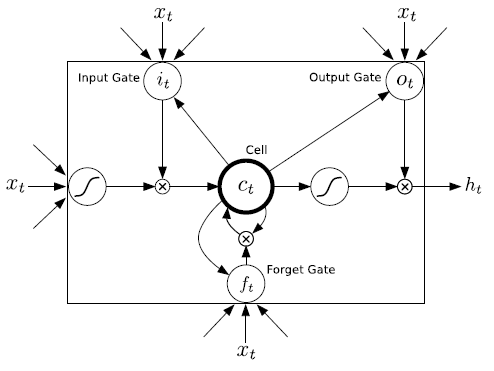
\includegraphics[width=7cm]{lstmcell}\\
  \caption{An LSTM Cell \cite{graves2013hybrid}}\label{fig_3_3_lstmcell}
\end{figure}

The gates in the above formula are illustrated in Figure \ref{fig_3_3_lstmcell}.  $\mathbf{i}_t$ represents the input gate, $\mathbf{f}_t$ is the forget gate and $\mathbf{o}_t$ represents the output gate.  At each of these gates therefore, the inputs consisting of hidden states in addition to the regular inputs are multiplied by a set of weights and passed through a soft-max function. These weights during training learn whether the gate will, during inference, open or not.  In summary, the input gate tells the LSTM whether or not to receive new information, the forget gate determines whether the current information it already has from the previous step should be kept or dropped and the output gate determines what should be forwarded to the next LSTM cell.  Note also that the LSTM has two sigmoid ($tanh$) activation functions utilised at the input and output of the current cell $\mathbf{c}_t$.

One particular variant of the original LSTM model is the GRU cell. Though simpler than an LSTM cell the GRU cell performs equally efficiently.  The main simplifications are that both state vectors are merged into a single vector $\mathbf{h}_{(t)}$. A single gate controller controls both the forget gate an the input gate.   If the gate controller outputs a 1, the input gate is open and the forget gate is closed.  If it outputs a 0, the opposite happens.  In other words, whenever a memory be stored, the location where it will be stored is erased first.  This is actually a frequent variant LSTM cell in and of itself. Finally, there is no output gate; the full vector cost is output at every time step.  However, there is a new gate controller that controls which part or the previous state will be shown to the main layer.

The overall architecture of a GRU is as follows:
\begin{equation}
\mathbf{z}_{(t)}=\sigma(\mathbf{W}_{xz}^T\cdot\mathbf{x}_{(t)}+\mathbf{W}_{hz}^T\cdot\mathbf{x}_{(t-1)})\label{eqn_c3_gru01}
\end{equation}
\begin{equation}
\mathbf{r}_{(t)}=\sigma(\mathbf{W}_{xr}^T\cdot\mathbf{x}_{(t)}+\mathbf{W}_{hr}^T\cdot\mathbf{x}_{(t-1)})\label{eqn_c3_gru01}
\end{equation}\begin{equation}
\mathbf{g}_{(t)}=\tanh(\mathbf{W}_{xg}^T\cdot\mathbf{x}_{(t)}+\mathbf{W}_{hg}^T\cdot(\mathbf{r}_{(t)}\otimes\mathbf{h}_{(t-1)}))\label{eqn_c3_gru01}
\end{equation}\begin{equation}
\mathbf{h}_{(t)}=(1-\mathbf{z}_{(t)})\otimes(\mathbf{h}_{(t-1)})+\mathbf{z}_{(t)}\otimes\mathbf{g}_{t}\label{eqn_c3_gru01}
\end{equation}

\section{Deep speech architecture}\label{deepspeech}

This work makes use of an enhanced RNN architecture called the Bi-directional Recurrent Neural Network (BiRNN). While \cite{hannun2014first} assert that forward recurrent connections does reflect the sequential relationships of an audio waveform, perhaps the BiRNN model poses a more powerful sequence model.

The BiRNN is a preferred end to end mechanism due to the length of sequence over which temporal relationships can be captured.  This implies that BiRNNs will be suited for capturing temporal relationships over much longer sequences than a forward only RNN, because hidden state information is preserved in both forwards and backwards direction. 

In addition, such a model has a notion of complete sentence or utterance  integration, having information over the entire temporal extent of the input features when making each prediction. 

The formulation of the BiRNN is derived by starting off with the basic RNN architecture which is referred to as the forward architecture.  From the forward architecture we derive the backward architecture. If we choose a temporally recurrent layer $j$, the BiRNN forward and backward intermediate hidden representation $h^{(f)}_t$ and $h^{(b)}_t$ is given as. 
\begin{equation}h_t^{(f)}=\sigma(\mathbf{W}^{(j)T}h_t^{(i-1)}+\mathbf{W}^{(f)T}_kh_{t-1}^{(j)}+b^{(j)}))
\label{eqn_c3_ds01}\end{equation}
\begin{equation}h_t^{(b)}=\sigma(\mathbf{W}^{(j)T}h_t^{(i-1)}+\mathbf{W}^{(b)T}_kh_{t+1}^{(b)}+b^{(j)}))
\label{eqn_c3_ds02}\end{equation}

Temporal weight matrices $W^{(f)}$ and $W^{(b)}$ propagate $h^{(f)}_t$  and $h^{(b)}_t$ forward and backward in time respectively. 

\cite{hannun2014first} points out that the recurrent forward and backward components are evaluated entirely independent of each other and for optimal training, a modified non linearity function $\sigma(z) = min(max(z, 0), 20)$ is recommended. 

The final BiRNN representation $h^{(j)}_t$ for the layer is now the sum of the two RNN components,
 \begin{equation}h_t^{(j)}=h_t^{(f)}+h_t^{(b)}
\label{eqn_c3_ds03}\end{equation}
Also note that back propagation sub gradient evaluations is computed from the combined BiRNN structure directly during training.

\subsection{Connectionist Temporal Classification (CTC)}
The term CTC stands for Connectionist Temporal classification.  This algorithm was designed to solve the problem of fuzzy alignment between the source input data and the output classification desired from the machine learning system.  This type of fuzzy alignment is observed in speech recognition systems as the same speech in either the same individual or different individuals will have different signal forms.  This is a many to one relationship between the input signal and the output classification that is dependent on the speaker style of speech when the utterance is spoken.  Unlike hybrid DNN-HMM networks the CTC algorithm deploys an end-to-end framework that models all aspects of the input sequence in a single neural network, therefore discarding the need for an HMM interpretation of the input sequence. In  addition, the CTC method does not require pre-segmented training data at the same time output classification is made independent of post-processing.

CTC works by making predictions at any point in the input sequence. For the case of speech modelling,  CTC makes a character prediction for every time step of the raw audio input speech signal. Although this initially seems counter intuitive, this method models the many to one relationship seen in the fuzzy audio speech to text alignment. 

For hybrid DNN-HMM systems, speech or more accurately, acoustic models, require separate training of targets for every time-slice in the input sequence. Secondly, and  as a consequence of this, it becomes necessary to segment the audio sequence, in order to provide targets for every time-slice. A third consequence is the limitation of DNNs previously discussed. As the DNN network only outputs local classifications, global aspects such as the likelihood of two consecutive labels appearing together cannot be directly modelled.  Without an external model, usually in the form of a language model, the hybrid speech model will significantly degrade performance.

In the CTC case, so long as the overall sequence of labels is correct the network can be optimised to correct the temporal or fuzzy alignments. Since this many to one fuzzy alignment is simultaneously modelled in CTC, then there is no need for pre-segmented data. At the same time, CTC models probabilities of complete label sequences, hence external post-processing required by hybrid models is eliminated.

Similar to the HMM sequence model, the CTC algorithm is a sequence model that predicts the next label in a sequence as a cumulative of previous sequences.  This section develops the CTC loss function borrowing concepts used in HMM models such as the forward backward algorithm as outlined in \citep{graves2006connectionist}.  In the following paragraph we introduce terminology associated with the CTC loss function.

Given two symbols $A$ and $\mathcal{B}$ such that $A$ has a many to one relationship with $\mathcal{B}$, signifying the temporal nature of the classification. The symbol $A$ represents an alphabet from which a sequence of the output classifications are drawn from. This CTC output consists of a soft-max layer in a BiRNN (bidirectional recurrent neural network). 

This output models the probability distribution of a complete sequence of arbitrary length $|A|$ over all possible labels in $A$ from activations within $|A|$. An extra activation is given to represent the probability of outputting a $blank$, or no label. At each time-step leading up to the final step, the probability distribution estimated as distribution over all possible label sequences of length leading up to that of the input sequence.

It is now possible to define the extended alphabet $A' = A \cup \{blank\}$, also, $y_{t,p}$ as the the activation of network output $p$ at time $t$.  Therefore $y_{t,p}$  is the probability that the network will output element $p \in A'$ at time $t$ given that $x$ is the input sequence of length $T$.  The distribution sought after $Pr(\pi|x)$, is the conditionally independent distribution over the subset $A'^T$ where $A'^T$ denotes the set of length $T$ sequences in $A'$. 
\begin{equation}
\Pr( \pi \, | \, x ) = \prod_{t=1}^{T} y_{t,\pi_t}
\label{eqn_c3_ctc01}\end{equation}

From the above, it is now possible to define the many-to-one mapping $\mathcal{B} : A'^T \rightarrow A^{\le T}$, from the set of paths onto the set $A^{\le T}$ of possible labellings of $x$ (i.e. the set of sequences of length less than or equal to $T$ over $A$). We do this by removing first the repeated labels and then the blanks from the paths. For example,

\begin{equation}\begin{aligned}\mathcal{B}(a - ab-) &= aab \\ \mathcal{B}(-aa - -abb) &= aab.\end{aligned} \label{eqn_c3_ctc02}
\end{equation}

Intuitively, this corresponds to outputting a new label when the network either switches from predicting no label to predicting a label, or from predicting one label to another. As $\mathcal{B}$ is many-to-one, the probability of some labelling $l \in A^{\le T}$ can be calculated by summing the probabilities of all the paths mapped onto it by $\mathcal{B}$:
\begin{equation}
\Pr( l \, | \, x) = \sum_{\pi \in \mathcal{B}^{-1}(l)} \Pr( \pi \, | \, x)
\label{eqn_c3_ct03}\end{equation}
This 'collapsing together' of different paths onto the same labelling is what makes it possible for CTC to use unsegmented data, because it allows the network to predict the labels without knowing in advance where they occur. In theory, it also makes CTC networks unsuitable for tasks where the location of the labels must be determined. However in practice CTC tends to output labels close to where they occur in the input sequence.

\subsection{Forward-backward algorithm}

The forward-backward algorithm is used to estimate the probability of a point in the sequence as the product of all point leading up to that point from the  initial state, the forward variable ($\alpha$), multiplied by the probability of all the points from that state to the end of the sequence, the backward variable ($\beta$).

The difference between this estimation and that determined from equation (\ref{eqn_c3_ct03}) is the fact that the forward-backward algorithm converts equation (\ref{eqn_c3_ct03}) into a form that is both recursive as well as reduces the computational complexity from an otherwise intractable computation to one that is readily computable.

With CTC, consider a modified "label sequence" $l'$, that caters for blank characters in between regular ones $l$, as defined in $A$. Thus, if $U$ is defined as the length of $l$.  Then $U'$ is of length $2U + 1$. CTC therefore integrates probability distributions of transitions between blank and non-blank labels at the same time CTC calculates those transition occurring between pairs of distinct non-blank labels.  The forward variable, $\alpha(t,u)$ now becomes the summed probability of all length $t$ paths that are mapped by $\mathcal{B}$ onto the length $\left \lfloor{u/2}\right \rfloor$ prefix of $l$. (Note, $\left \lfloor{u/2}\right \rfloor$ is the floor of $u/2$, the greatest integer less than or equal to $u/2$.) For some sequence $s$, let $s_{p:q}$ denote the sub-sequence $s_p, s_{p+1},\dots,s_{q-1},s_q$, and define the set $V(t,u) \equiv \{ \pi \in A'^t : \mathcal{B}(\pi) = l_{1:\left \lfloor{u/2}\right \rfloor} \text{ and } \pi_t = l'_u \}$.  $\alpha(t,u)$ then becomes
\begin{equation}
\alpha(t,u) \equiv \sum_{\pi \in V(t,u)} \prod_{i=1}^{t} y_{i,\pi_i} 
\label{eqn_c3_ctc04}
\end{equation}

The forward variables at time $t$ can be calculated recursively from those at time $t - 1$ and expressed as the sum of the forward variables with and without the final blank at time $T$.

\begin{equation}
\Pr( l \, | \, x) = \alpha(T, U') + \alpha(T, U' - 1)
\label{eqn_c3_ctc05}
\end{equation}

All correct paths must start with either a blank $(b)$ or the first symbol in $l$ $(l_1)$, yielding the following initial conditions:
\begin{equation}
\begin{aligned}\alpha(1, 1) &= y_{1,b} \\ \alpha(1, 2) &= y_{1,l_1} \\ \alpha(1, u) &= 0, \, \forall u > 2 \end{aligned}
\label{eqn_c3_ctc05}\end{equation}

Thereafter the variables can be calculated recursively:
\begin{equation}
\alpha(t,u) = y_{t, l'_u} \sum_{i = f(u)}^{u} \alpha(t-1, i)
\label{eqn_c3_ctc06}\end{equation}
where
\begin{equation}
f(u) =\begin{cases}u-1, & \text{ if } l'_u = blank \text{ or } l'_{u-2} = l'_{u} \\ u-2, & \text{otherwise}\end{cases}
\label{eqn_c3_ctc07}\end{equation}
Graphically we can express the recurrence relation for $\alpha(t, u)$ as follows.

\begin{figure}
\centering
  % Requires \usepackage{graphicx}
  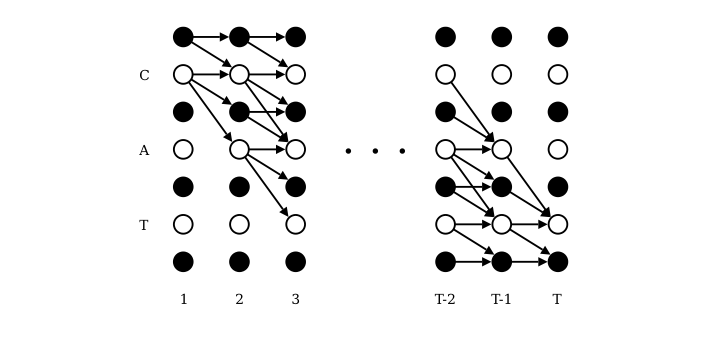
\includegraphics[width=9cm]{thesis/images/Lattice.png}
  \caption{Beam Search Lattice Structure \citep{graves2006connectionist}}
\label{fig_3_a_lattice}
\end{figure}

where $t$ runs along the $x$ axis and $u$ runs along the $y$ axis. The black circles of the diagram represent $blank$ elements of $l'$ while the white circles represent non-$blank$ elements of $l'$. The arrows represent computational dependencies derived from our recursion relation for $\alpha(t,u)$. So, for example, the value of $\alpha(2,3)$, corresponding to the $blank$ at $t=2$ and $u=3$, is derived from $\alpha(1,2)$. Similarly, the value of $\alpha(2,2)$, corresponding to the letter $c$ at $t=2$ and $u=2$, is derived from $\alpha(1,2)$ and $\alpha(1,1)$.
\begin{equation}
\alpha(t,u)=0 \quad \forall u < U'-2(T-t)-1
\label{eqn_c3_ctc07}\end{equation}
because these variables correspond to states for which there are not enough time-steps left to complete the sequence. We also impose the boundary condition
\begin{equation}
\alpha(t, 0) = 0 \quad \forall t
\label{eqn_c3_ctc08}
\end{equation}
The backward variables $\beta(t,u)$ are defined as the summed probabilities of all paths starting at $t + 1$ that "complete" $l$ when appended to any path $\hat{\pi}$ contributing to $\alpha(t,u)$. Define $W(t,u) \equiv \{ \pi \in A'^{T-t} : \mathcal{B}(\hat{\pi} + \pi) = l \, \, \forall \hat{\pi} \in V(t,u) \}$. Then
\begin{equation}
\beta(t,u) \equiv \sum_{\pi \in W(t,u)} \prod_{i=1}^{T - t} y_{t + i,\pi_i} \label{eqn_c3_ctc08}\end{equation}

The rules for initialisation of the backward variables are as follows
\begin{equation} \begin{aligned}
\beta(T, U') &= 1 \\
\beta(T, U' - 1) &= 1 \\
\beta(T, u) &= 0, \, \forall u < U' - 1
\end{aligned}\label{eqn_c3_ctc09}\end{equation}

The rules for recursion are as follows:
\begin{equation}
\beta(t, u) = \sum_{i = u}^{g(u)} \beta(t+1, i) y_{t+1, l'_i}\label{eqn_c3_ctc10}\end{equation}
where
\begin{equation}
g(u) = \begin{cases} u + 1,& \text{if } l'_u = blank \text{ or } l'_{u+2} = l'_{u} \\ u + 2,& \text{otherwise} \end{cases}   
\end{equation}

\subsection{CTC Loss function}

The cross entropy error is a loss function used to measure accuracy of probabilistic measures.  It is calculated as the negative log probability of a likelihood measure.  The CTC loss function $\mathcal{L}(S)$ uses the cross entropy loss function of and is defined as the cross entropy error of correctly labelling all the training samples in some training set S:
\begin{equation}
\mathcal{L}(S) = - \ln \prod_{(x,z) \in S} \Pr(z \, | \, x) = - \sum_{(x,z) \in S} \ln \Pr(z \, | \, x)
\label{eqn_c3_ctc11}\end{equation}
where $z$ is the output label and $x$ is the input sequence.  Since $\mathcal{L}(S)$ in equation \ref{eqn_c3_ctc11} is differentiable, this loss function can be back propagated to the softmax layer in the BiRNN configuration discussed in section \ref{deepspeech}.
\begin{equation}
\mathcal{L}(x,z) \equiv - \ln \Pr(z \, | \, x)
\label{eqn_c3_ctc12}\end{equation}
and therefore 
\begin{equation}
\mathcal{L}(S) = \sum_{(x,z) \in S} \mathcal{L}(x,z)
\label{eqn_c3_ctc12}\end{equation}

From the definition of the forward and backward variables ($\alpha(t, u)$ and $\beta(t, u)$), we also establish that $X(t,u) \equiv \{ \pi \in A'^T : \mathcal{B}(\pi) = z, \, \pi_t = z'_u \}$, such that
\begin{equation}
\alpha(t, u) \beta(t, u) = \sum_{\pi \in X(t,u)} \prod_{t = 1}^{T} y_{t, \pi_t}\label{eqn_c3_ctc13}\end{equation}

then substituting $\Pr(\pi \, | \, x)$ from the expression in equation \ref{eqn_c3_ctc01}, we have
\begin{equation}
\alpha(t, u) \beta(t, u) = \sum_{\pi \in X(t,u)} \Pr(\pi \, | \, x)
\label{eqn_c3_ctc14}\end{equation}

Also observe that $\Pr(l \, | \, x)$ is equivalent to the total probability $\Pr(z \, | \, x)$. Paths going through $z'_u$ at time $t$ can be obtained as summed over all $u$ to get
\begin{equation}
\Pr(z \, | \, x) = \sum_{u = 1}^{|z'|} \alpha(t, u) \beta(t, u)
\label{eqn_c3_ctc15}\end{equation}

Thus a sample loss is determined by
\begin{equation}
\mathcal{L}(x, z) = - \ln \sum_{u = 1}^{|z'|} \alpha(t, u) \beta(t, u)\label{eqn_c3_ctc16}
\end{equation}
and therefore the overall loss is given by
\begin{equation}\mathcal{L}(S) = -\sum_{(x,z) \in S} \ln \sum_{u = 1}^{|z'|} \alpha(t, u) \beta(t, u)
\label{eqn_c3_ctc17}\end{equation}

In the model described in this work, the gradient $\mathcal{L}(x, z)$is computed using TensorFlow's automatic differentiation capabilities. In practice, computations soon lead to underflow however the log scale, being used in the above loss function calculations avoids this situation and another useful equation in this context is
\begin{equation}
\ln(a + b) = \ln(a) + \ln(1 + e^{\ln b - \ln a})
\label{eqn_c3_ctc18}\end{equation}
